\section{Aspetti riprodotti}
\begin{frame}{Indicizzazione e LM}
    \begin{columns}
        \begin{column}{0.5\textwidth}
            \begin{itemize}
                \item Lucene... Quale versione?
            \end{itemize}
            \bigskip
            \begin{itemize}
                \item Indicizzazione... In che modo?
                      \begin{itemize}
                          \item Tokenizing
                          \item Rimozione stopword
                          \item Indice trasposto
                      \end{itemize}
            \end{itemize}
            \bigskip
            \begin{itemize}
                \item Base Language Model
            \end{itemize}
        \end{column}
        \begin{column}{0.5\textwidth}

            \bigskip
            
\includegraphics[width=\columnwidth]{img/lucene_logo.png}
            
            \bigskip
            \bigskip
            \bigskip
            \bigskip
            \bigskip
            \bigskip
            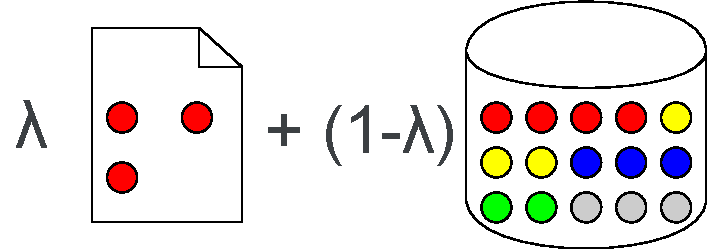
\includegraphics[width=\columnwidth]{img/lm.pdf}
        \end{column}
    \end{columns}
\end{frame}

\begin{frame}{GLM}
    \begin{center}
        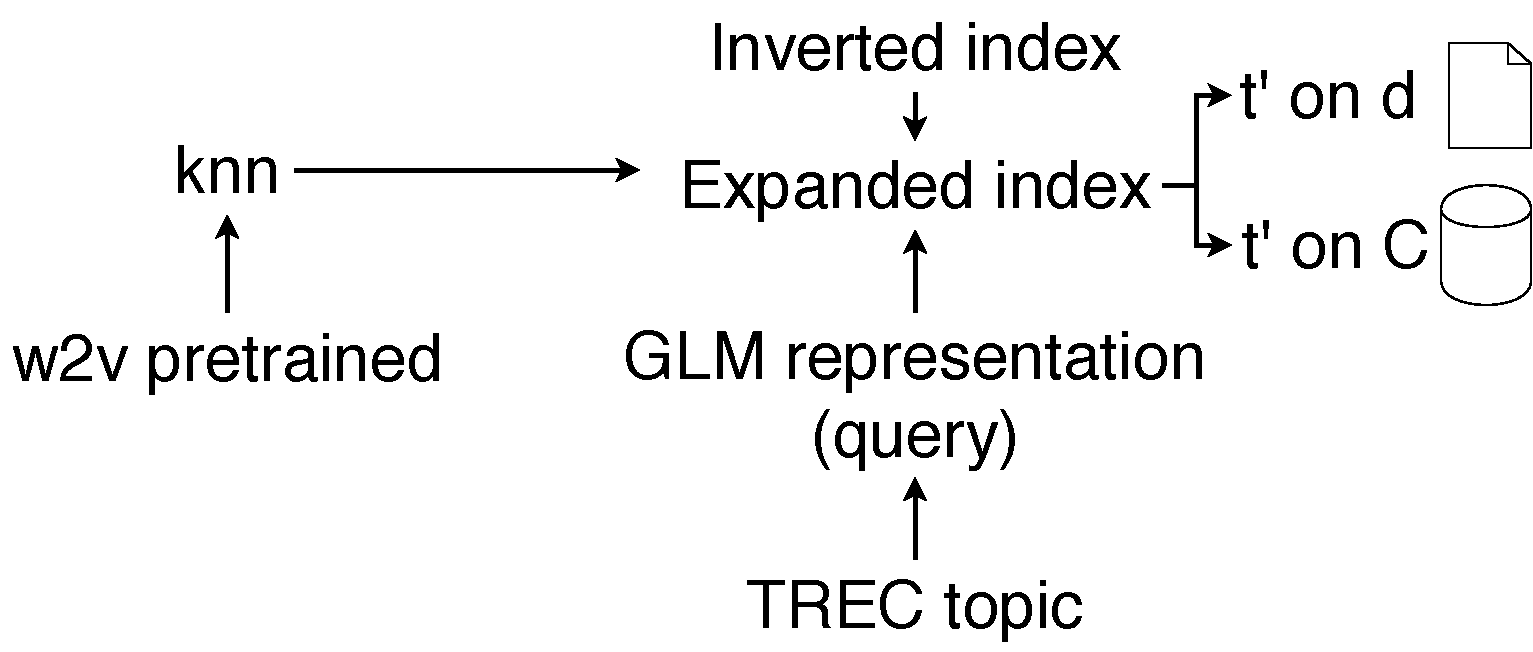
\includegraphics[width=0.8\textwidth]{img/reproduction.pdf}
    \end{center}
    \begin{columns}
        \begin{column}{0.33\textwidth}
            \begin{itemize}
                \item Primo approccio: chi fa da sè... Fa da sè!
            \end{itemize}
        \end{column}
        \begin{column}{0.33\textwidth}
            \begin{itemize}
                \item Secondo approccio: cerchiamo di prendere esempio e di migliorare
            \end{itemize}
        \end{column}
        \begin{column}{0.33\textwidth}
            \begin{itemize}
                \item È abbastanza? No, per vincoli di tempo...
            \end{itemize}
        \end{column}
    \end{columns}
\end{frame}
